\documentclass[a4paper, 12pt]{article}

\usepackage{cmap}
\usepackage{mathtext} 
\usepackage[T2A]{fontenc}
\usepackage[utf8]{inputenc}
\usepackage[english,russian]{babel}	

\usepackage{amsfonts,amssymb,amsthm,mathtools}
\usepackage{amsmath}
\usepackage{icomma} 

\usepackage{graphicx} 
\graphicspath{{Picturies/}}
\usepackage{wrapfig}

\usepackage{array,tabularx,tabulary,booktabs}
\usepackage{longtable}
\usepackage{multirow}

\usepackage{caption}
\captionsetup{labelsep=period}

\renewcommand{\phi}{\varphi}
\newcommand{\eps}{\varepsilon}
\renewcommand{\AA}{\ensuremath{\mathring{A}}}
\newcommand{\parag}[1]{\paragraph*{#1:}}

\newcounter{Points}
\setcounter{Points}{1}
\newcommand{\point}{\arabic{Points}. \addtocounter{Points}{1}}

\author{Вязовцев Андрей, Б01-009}
\date{19.10.22}
\title{Лабораторная работа 5.1.3. Изучение рассеяния медленных электронов на атомах (эффект Рамзауэра).}

\begin {document}

\maketitle

\parag {Цель работы}  Исследуется энергетическая зависимость вероятности рассеяния электронов атомами ксенона, определяются энергии электронов, при которых наблюдается <<просветление>> ксенона, и оценивается размер его внешней электронной оболочки. 

\parag {В работе используются} тиратрон ТГ3-01/1.3Б

\parag {Теоретическая справка} ~\\

Эффективное сечение реакции --- величина, характеризующая вероятность перехода системы двух сталкивающихся частиц в результате их рассеяния в определённое конечное состояние.

\begin{equation}
    \sigma = \frac{N}{nv}
\end{equation}

Если построить зависимость $\sigma (E)$, то получится график как на рис. \ref{pic:sigE}.

\begin{figure}[!h]
    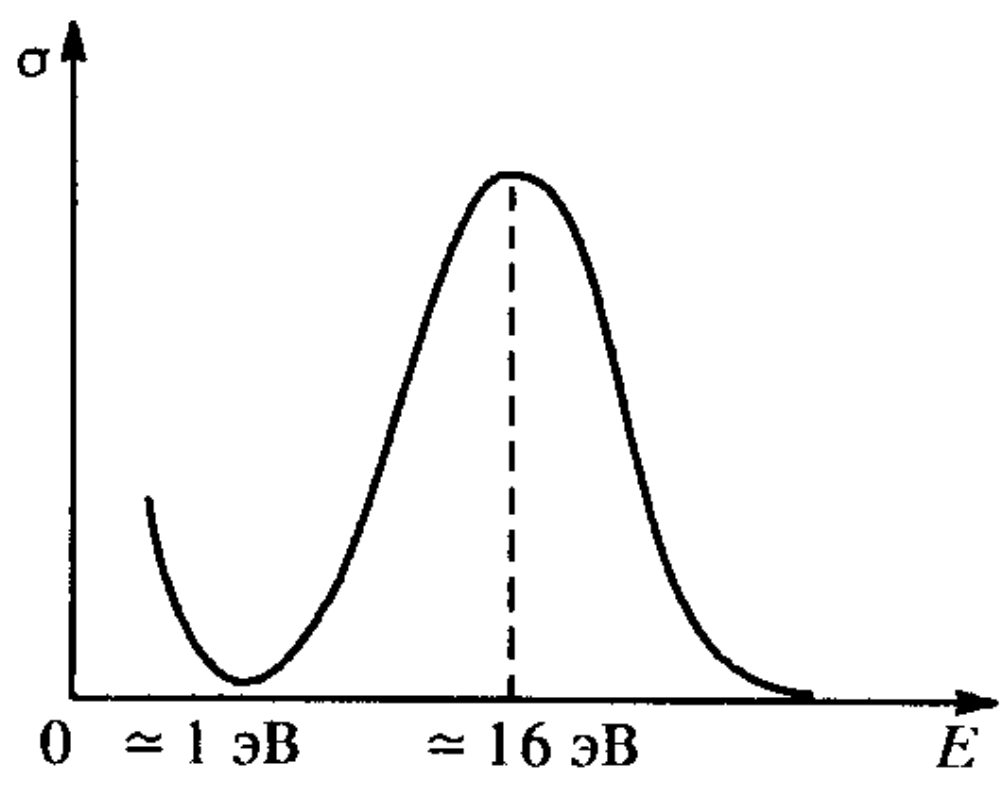
\includegraphics[scale = 0.3]{sig_e}
    \centering
    \caption{Качественная картина результатов измерения упругого рассеяния электронов в аргоне}
    \label{pic:sigE}
\end{figure}

Отсюда видно, что при энергии 1 эВ есть <<прозрачное окно>>, т.е. электроны свободно проходят через среду аргона. Такое явление нельзя объяснить с помощью классической физики. По отношению к электронной волне атом ведёт себя как преломляющая волна:

\begin{equation}
    n = \frac{\lambda}{\lambda^\prime} = \sqrt{1 - \frac{U}{E}}
\end{equation}

Решение задачи о рассеянии электрона на сферической потенциальной яме достаточно громоздко, поэтому в нашей модели будем считать, что яма является одномерной конечной глубины $U_0$ шириной $l$. Используя уравнение Шрёдингера и вычисляя коэффициент прохождения, получаем условие на его максимумы:

\begin{equation}
    k_2 l = \sqrt{\frac{2 m (E + U)}{\hbar^2}}l = \pi n, ~ n \in \mathbb{N} 
\end{equation}

Для качественного объяснения эффекта Рамзауэра достаточно использовать соотношение де Бройля и рассмотреть интерференцию волн ле Бройля в атоме. Условие максимума: разность хода равна длине волны в атоме:

\begin{equation}
    2l = \lambda_1 = \frac{h}{\sqrt{2 m (E_1 + U_0)}}
    \label{eq:max}
\end{equation}

Здесь $E_1$ --- энергия, соответствующая данному условию. С другой стороны, можно таким же образом найти минимум:

\begin{equation}
    2l = \frac{3}{2} \lambda_2 = \frac{3}{2} \frac{h}{\sqrt{2 m (E_2 + U_0)}}
    \label{eq:min}
\end{equation}

Решив эти уравнения, исключаем $U_0$ и получаем:

\begin{equation}
    l = \frac{h \sqrt{5}}{\sqrt{32 m (E_2 - E_1)}}
    \label{eq:without_U}
\end{equation}

Понятно, что энергии $E_1$ и $E_2$ соответствуют энергиям электронов, прошедших разность потенциалов, т.~е. $E_1 = e V_1$, $E_2 = e V_2$. Из уравнений \eqref{eq:max} и \eqref{eq:min} можно получить глубину ямы:

\begin{equation}
    U_0 = \frac{4}{5} E_2 - \frac{9}{5} E_1
    \label{eq:U}
\end{equation}

\parag {Экспериментальная установка} ~

В данной работе для изучения эффекта Рамзауэра используется тиратрон ТГ3-01/1.3Б (см. рис. \ref{pic:work1}). В нём:

\begin{itemize}
    \item 1, 2, 3 --- сетки
    \item 4 --- внешний металлический цилиндр
    \item 5 --- катод
    \item 6 --- анод
    \item 7 --- накаливаемая спираль
\end{itemize}

Уравнение ВАХ выражается так:

\begin{equation}
    I_a = I_0 e^{-C \omega(V)}
\end{equation}

где $I_0 = eN_0$ --- ток катода, $I_а = e N_a$ --- анодный ток, $C = L n_а \Delta_а$, $L$ --- расстояние от катода до анода, $n_a$ --- концентрация атомов газа в лампе, $\Delta_a$ --- площадь поперечного сечения атома, $\omega (V)$ --- вероятность рассеяния на атоме. Отсюда вероятность выражается так:

\begin{equation}
    \omega (V) = - \frac{1}{C} \ln \frac{I_a(V)}{I_0}
    \label{eq:prob}
\end{equation}

\begin{figure}[!h]
    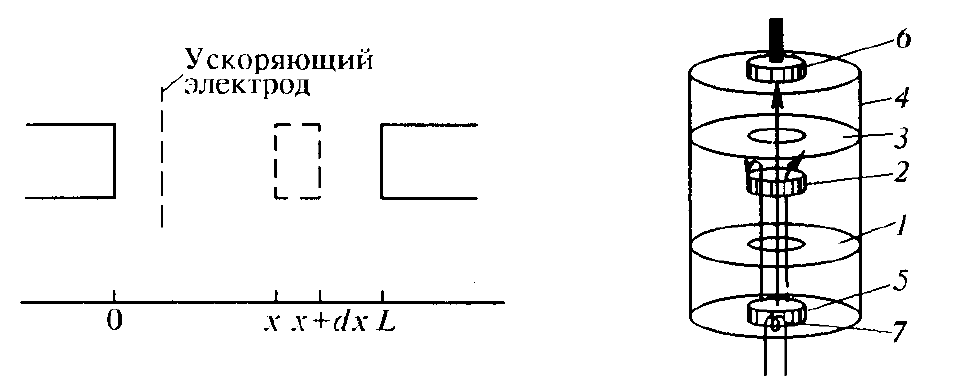
\includegraphics[scale = 0.4]{Workplace1}
    \centering
    \caption{Схема тиратрона (слева) и его конструкция (справа)}
    \label{pic:work1}
\end{figure}

\begin{figure}[!h]
    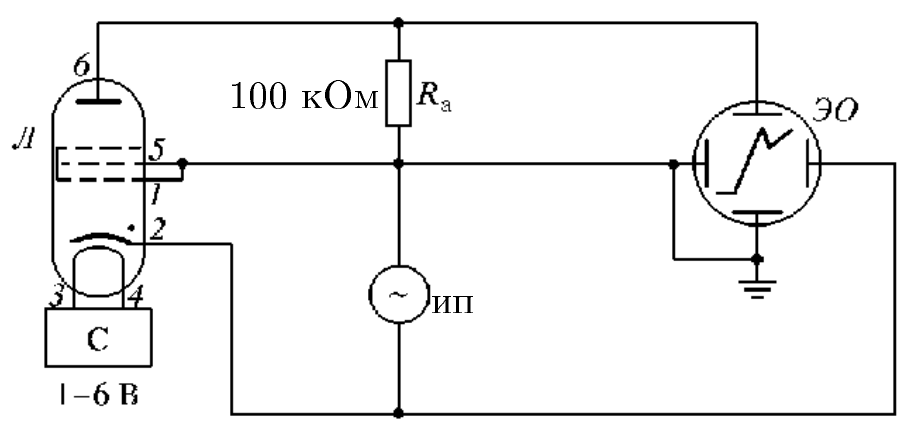
\includegraphics[scale = 0.4]{Workplace2}
    \centering
    \caption{Схема включения тиратрона}
    \label{pic:work2}
\end{figure}

\begin{figure}[!h]
    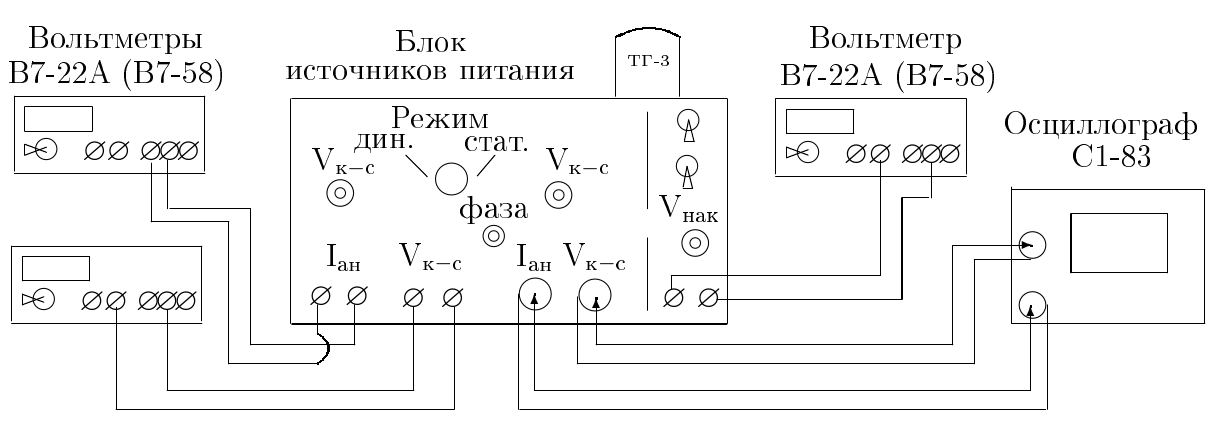
\includegraphics[scale = 0.4]{Workplace3}
    \centering
    \caption{Блок-схема экспериментальной установки}
    \label{pic:work3}
\end{figure}

\newpage

\parag {Ход работы} ~\\

\point Подготовим осциллограф к работе, затем включим в сеть.

\point Поставим переключатель в динамический режим. Измерим с помощью осциллографа напряжение в точках максимума, минимума и пробоя. Результаты представлены в таблице \ref{tab:dyn}, а осциллограммы --- на рисунках \ref{pic:dyn1} и \ref{pic:dyn2}.

\begin{table}[!h]
    \centering
    \begin{tabular}{|c|c|c|c|c|c|}
        \hline
        $U_{нак}$, В & $V_{max}$, В & $V_{min}$, В & $V_{пр}$, В \\ \hline
        $2.839$ & $1.3 \pm 0.1$ & $2.8 \pm 0.2$ & $5.4 \pm 0.4$ \\ \hline
        $3.125$ & $1.5 \pm 0.1$ & $3.2 \pm 0.2$ & $5.1 \pm 0.1$ \\ \hline
    \end{tabular}
    \caption {Данные с осциллограммы}
    \label{tab:dyn}
\end{table}

\begin{figure}[!h]
    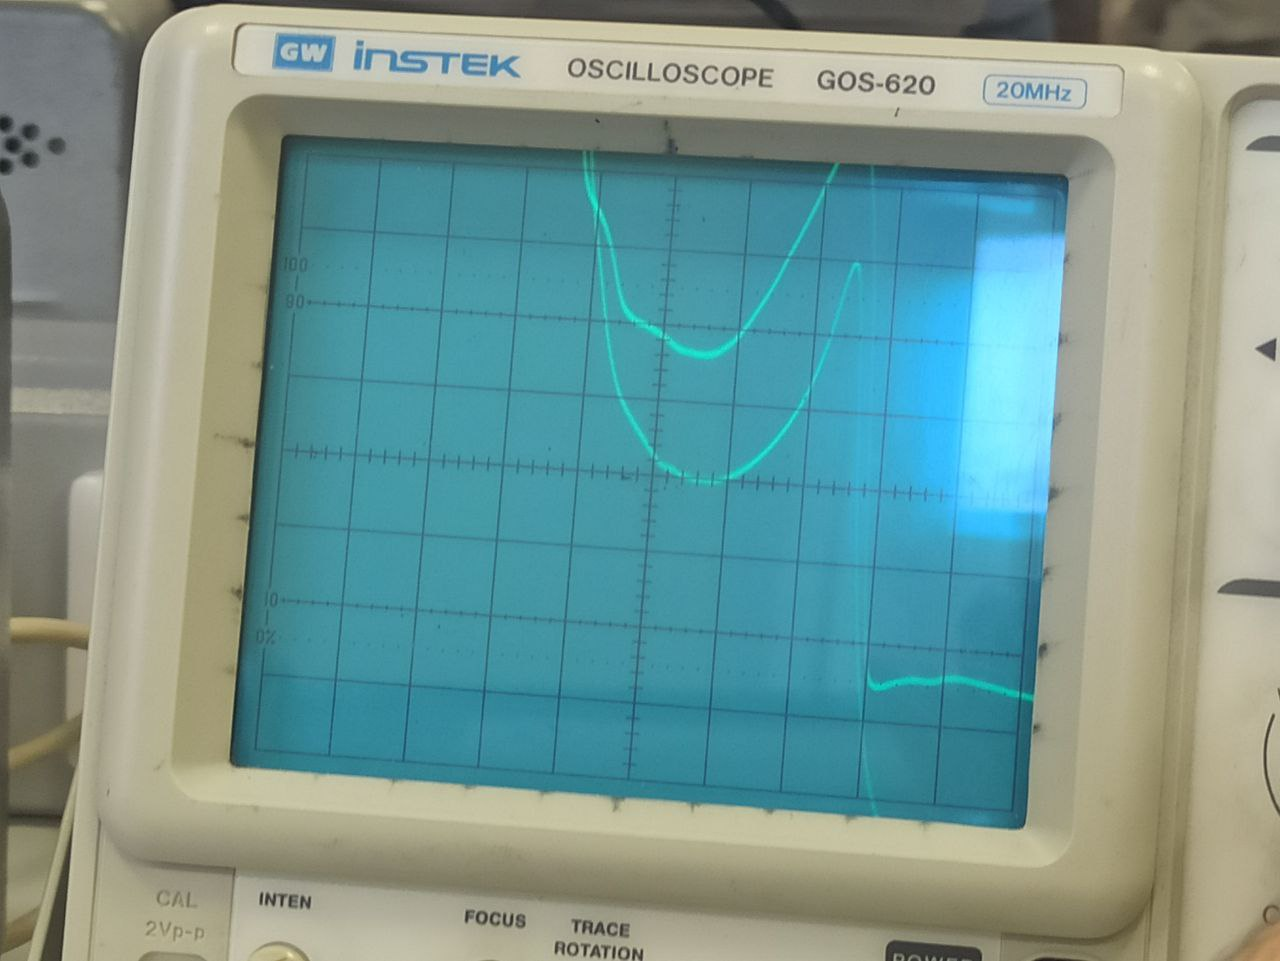
\includegraphics[scale = 0.2]{dyn1}
    \centering
    \caption{}
    \label{pic:dyn1}
\end{figure}

\begin{figure}[!h]
    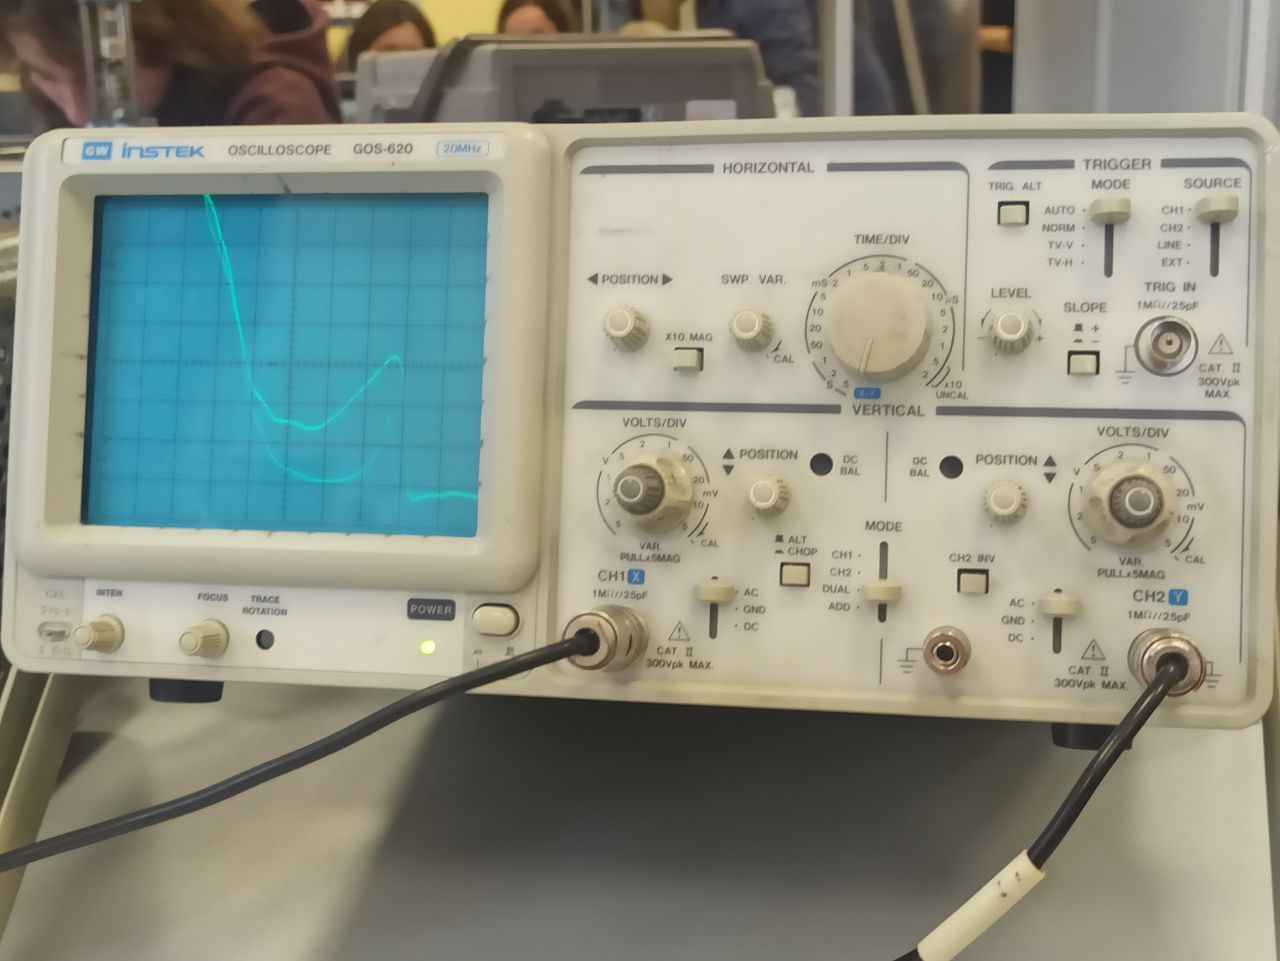
\includegraphics[scale = 0.2]{dyn2}
    \centering
    \caption{}
    \label{pic:dyn2}
\end{figure}

\newpage

\point Теперь переключим в статический режим. Измерим ток анода, изменяя катода с промежутком $0.5$ В при тех же $U_{нак}$. Результаты для $U_{нак} = 2.844$ В представлены в таблице \ref{tab:stat1}, а для $U_{нак} = 3.169$ --- в таблице \ref{tab:stat2}.

\begin{table}[!h]
    \centering
    \begin{tabular}{|c|c|c|c|c|c|c|c|c|c|c|}
        \hline
        $V_{кат}$, В & 1.000 & 1.500 & 2.000 & 2.553 & 3.097 & 3.602 & 4.030 & 4.509 & 5.019 & 5.498 \\ \hline
        $V_{ан}$, В & 0.00 & 0.38 & 30.80 & 50.50 & 37.23 & 32.50 & 30.33 & 28.52 & 26.83 & 25.58 \\ \hline
    \end{tabular}
    ~\\
    \begin{tabular}{|c|c|c|c|c|c|c|c|c|c|c|}
        \hline
        $V_{кат}$, В & 6.027 & 6.521 & 7.046 & 7.515 & 8.007 & 8.499 & 9.024 & 9.516 & 10.078 & 2.200 \\ \hline
        $V_{ан}$, В & 24.66 & 24.11 & 23.79 & 23.78 & 24.1 & 25.02 & 26.22 & 26.71 & 28.18 & 49.10 \\ \hline
    \end{tabular}
    ~\\
    \begin{tabular}{|c|c|c|c|c|c|c|}
        \hline
        $V_{кат}$, В & 2.298 & 2.400 & 2.488 & 2.821 & 7.215 & 7.408 \\ \hline
        $V_{ан}$, В & 52.56 & 52.90 & 51.92 & 43.83 & 24.12 & 23.91 \\ \hline
    \end{tabular}
    \caption {Измерения для $U_{нак} = 2.844$}
    \label{tab:stat1}
\end{table}

\begin{table}[!h]
    \centering
    \begin{tabular}{|c|c|c|c|c|c|c|c|c|c|c|}
        \hline
        $V_{кат}$, В & 1.000 & 1.500 & 2.077 & 2.516 & 3.036 & 3.501 & 4.026 & 4.511 & 5.037 & 5.507 \\ \hline
        $V_{ан}$, В & 0.00 & 1.10 & 66.77 & 98.07 & 91.69 & 86.95 & 82.52 & 78.47 & 74.28 & 70.87 \\ \hline
    \end{tabular}
    ~\\
    \begin{tabular}{|c|c|c|c|c|c|c|c|c|c|c|}
        \hline
        $V_{кат}$, В & 6.047 & 6.497 & 7.014 & 7.539 & 8.016 & 8.511 & 9.014 & 9.500 & 10.048 & 2.207 \\ \hline
        $V_{ан}$, В & 68.81 & 67.74 & 67.15 & 67.52 & 68.99 & 71.66 & 75.45 & 77.99 & 82.00 & 84.42 \\ \hline
    \end{tabular}
    ~\\
    \begin{tabular}{|c|c|c|c|c|c|c|c|c|}
        \hline
        $V_{кат}$, В & 2.293 & 2.427 & 2.600 & 2.785 & 7.214 & 7.415 & 7.717 & 7.923 \\ \hline
        $V_{ан}$, В & 90.93 & 95.57 & 95.90 & 94.17 & 70.19 & 70.94 & 72.05 & 72.85 \\ \hline
    \end{tabular}
    \caption {Измерения для $U_{нак} = 3.169$}
    \label{tab:stat2}
\end{table}

\newpage

\parag {Обработка результатов} ~\\

\point Примем $U_0 = 2.5$ эВ и найдём размер электронной оболочки атома по результатам измерений в динамическом режиме по формулам \eqref{eq:max} и \eqref{eq:min}. Получаем:

\begin{table}[!h]
    \centering
    \begin{tabular}{|c|c|c|}
        \hline
        $U_{нак}$ & l по формуле \eqref{eq:max} & l по формуле \eqref{eq:min} \\ \hline
        $2.829$ & $1.00 \pm 0.08$ \AA & $1.26 \pm 0.09$ \AA \\ \hline
        $3.125$ & $0.97 \pm 0.06$ \AA & $1.22 \pm 0.08$ \AA \\ \hline
    \end{tabular}
\end{table}

Теперь вычислим данный размер по формуле \eqref{eq:without_U}. Получаем:

\begin{align*}
    l &= 1.77 \pm 0.18 \text{ \AA, при } U_{нак} = 2.829 \\
    l &= 1.66 \pm 0.15 \text{ \AA, при } U_{нак} = 3.125
\end{align*}

\point Найдём глубину потенциальной ямы по формуле \eqref{eq:U}:

\begin{align*}
    U_0 &= -0.1 \pm 0.3 \text{ эВ, при } U_{нак} = 2.829 \\
    U_0 &= -0.1 \pm 0.3 \text{ эВ, при } U_{нак} = 3.125
\end{align*}

Комментировать данные результаты мы не будем. Это какой-то волшебный газ.

\point Построим графики $I_a = f(V_c)$ для статического режима. Учтём, что $I_a = V_a / R_a$, где $R_a = 100$ кОм. Теперь вычислим все величины, которые вычисляли для динамического режима:

\begin{table}[!h]
    \centering
    \begin{tabular}{|c|c|c|c|c|}
        \hline
        $U_{нак}$ & $U_{max}$ & $U_{min}$ & l по формуле \eqref{eq:max} & l по формуле \eqref{eq:min} \\ \hline
        $2.829$ & $2.3 \pm 0.1$ В & $7.3 \pm 0.1$ В & $0.89 \pm 0.04$ \AA & $0.93 \pm 0.01$ \AA \\ \hline
        $3.125$ & $2.5 \pm 0.1$ В & $7.2 \pm 0.2$ В & $0.87 \pm 0.03$ \AA & $0.93 \pm 0.03$ \AA \\ \hline
    \end{tabular}
    ~\\ ~\\
    \begin{tabular}{|c|c|c|}
        \hline
        $U_{нак}$ & l по формуле \eqref{eq:without_U} & $U_0$ \\ \hline
        $2.829$ & $0.97 \pm 0.04$ \AA & $1.7 \pm 0.3$ эВ \\ \hline
        $3.125$ & $1.00 \pm 0.05$ \AA & $1.3 \pm 0.4$ эВ \\ \hline
    \end{tabular}
\end{table}

\begin{figure}[!h]
    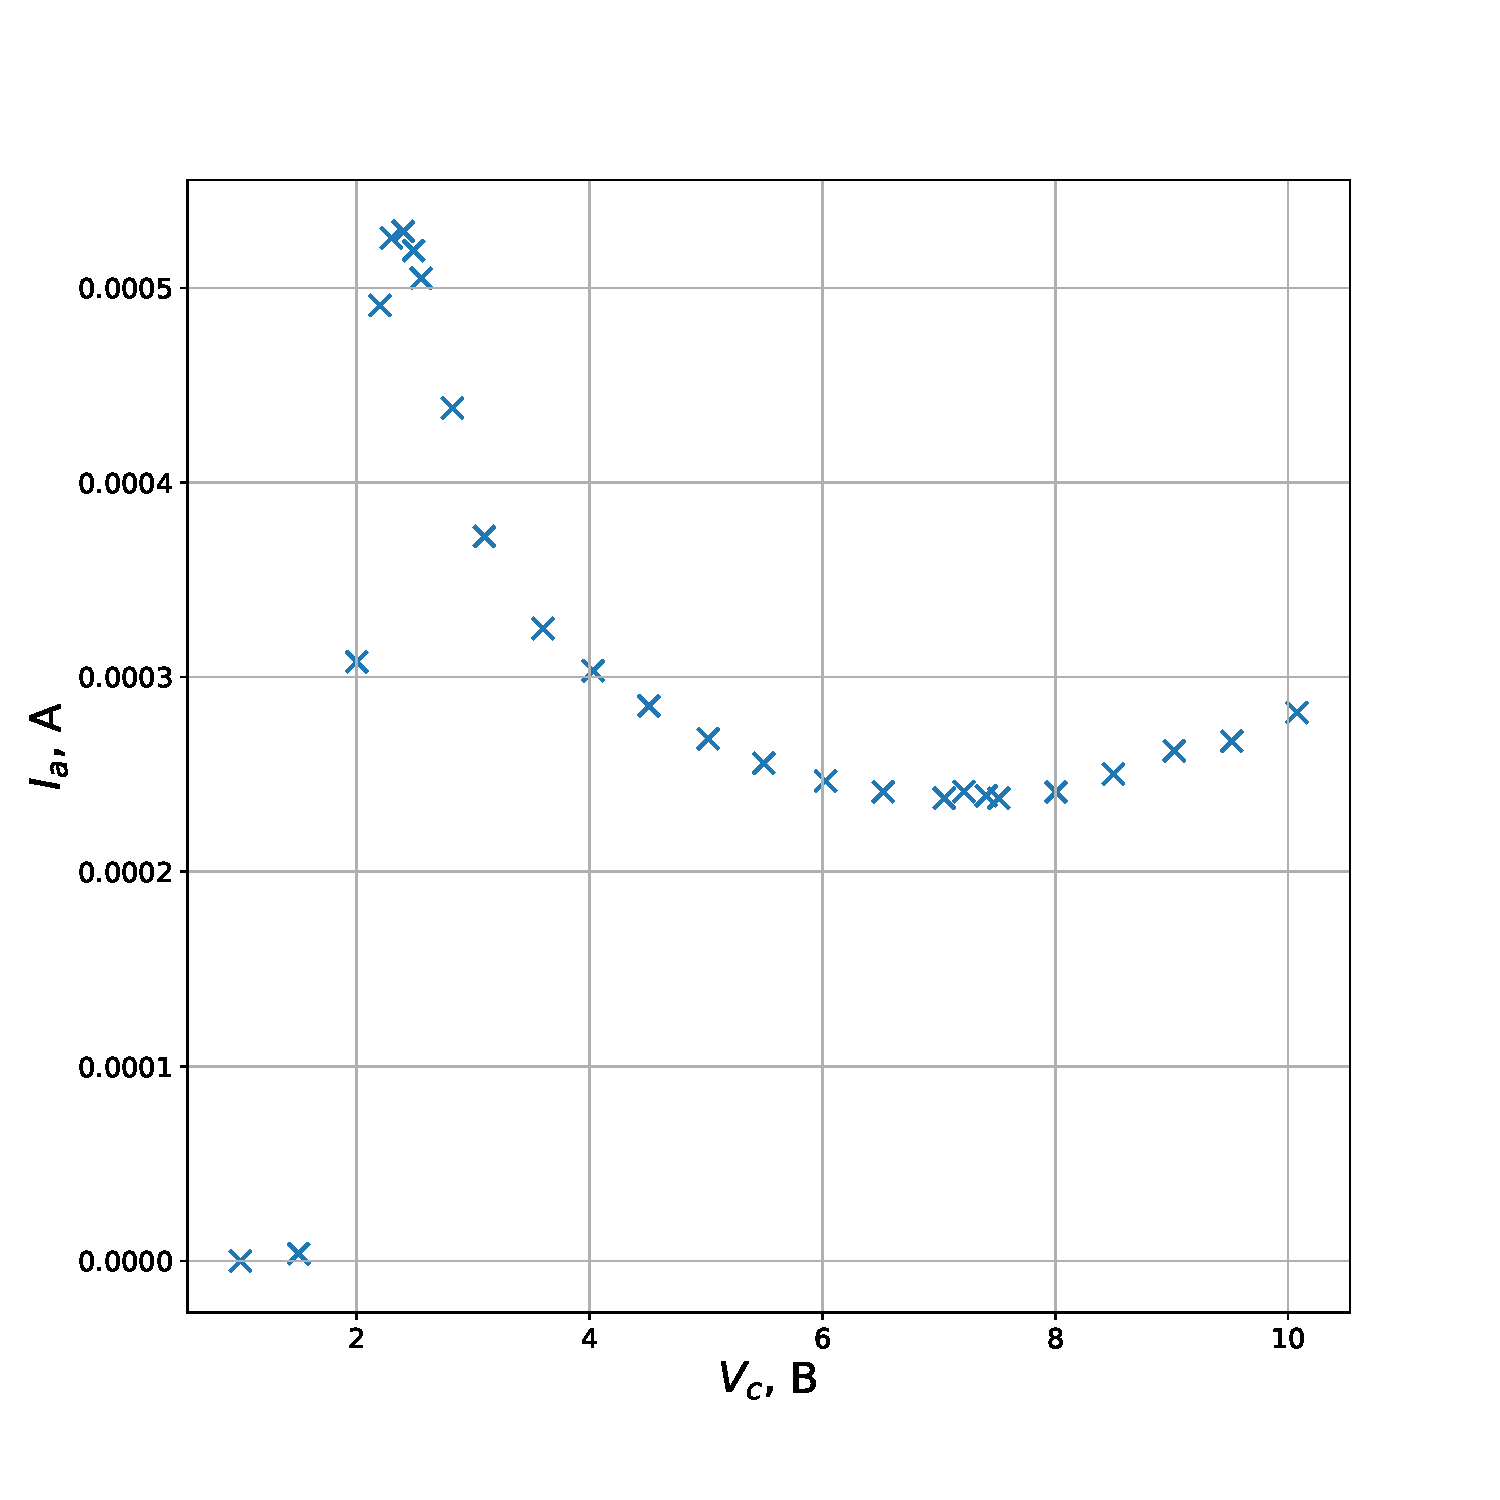
\includegraphics[scale = 0.4]{graph1}
    \centering
    \caption{$U_{нак} = 2.829$}
    \label{pic:graph1}
\end{figure}

\begin{figure}[!h]
    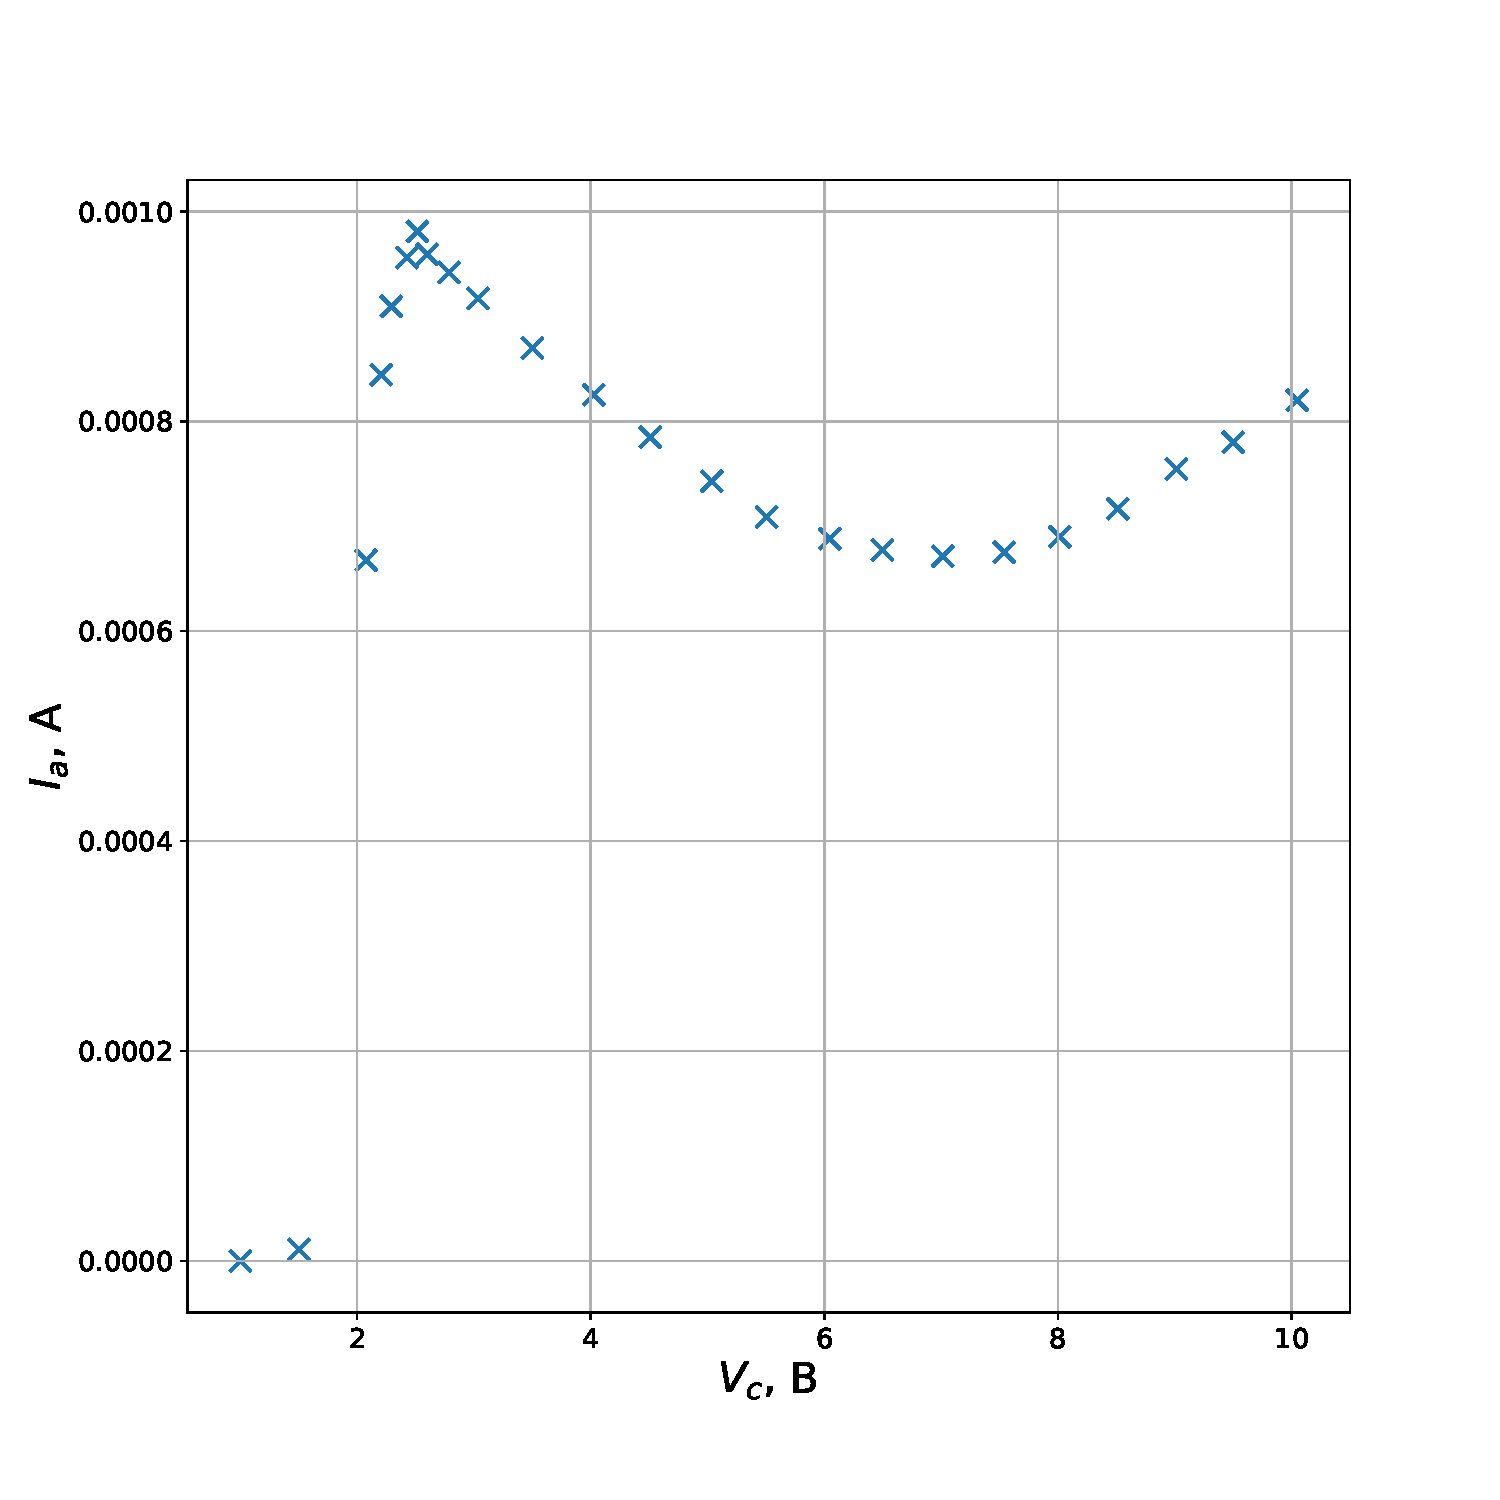
\includegraphics[scale = 0.36]{graph2}
    \centering
    \caption{$U_{нак} = 3.125$}
    \label{pic:graph2}
\end{figure}

\point На основе формулы \eqref{eq:prob} найдём вероятности рассеяния электронов и построим соответствующий график.

\begin{figure}[!h]
    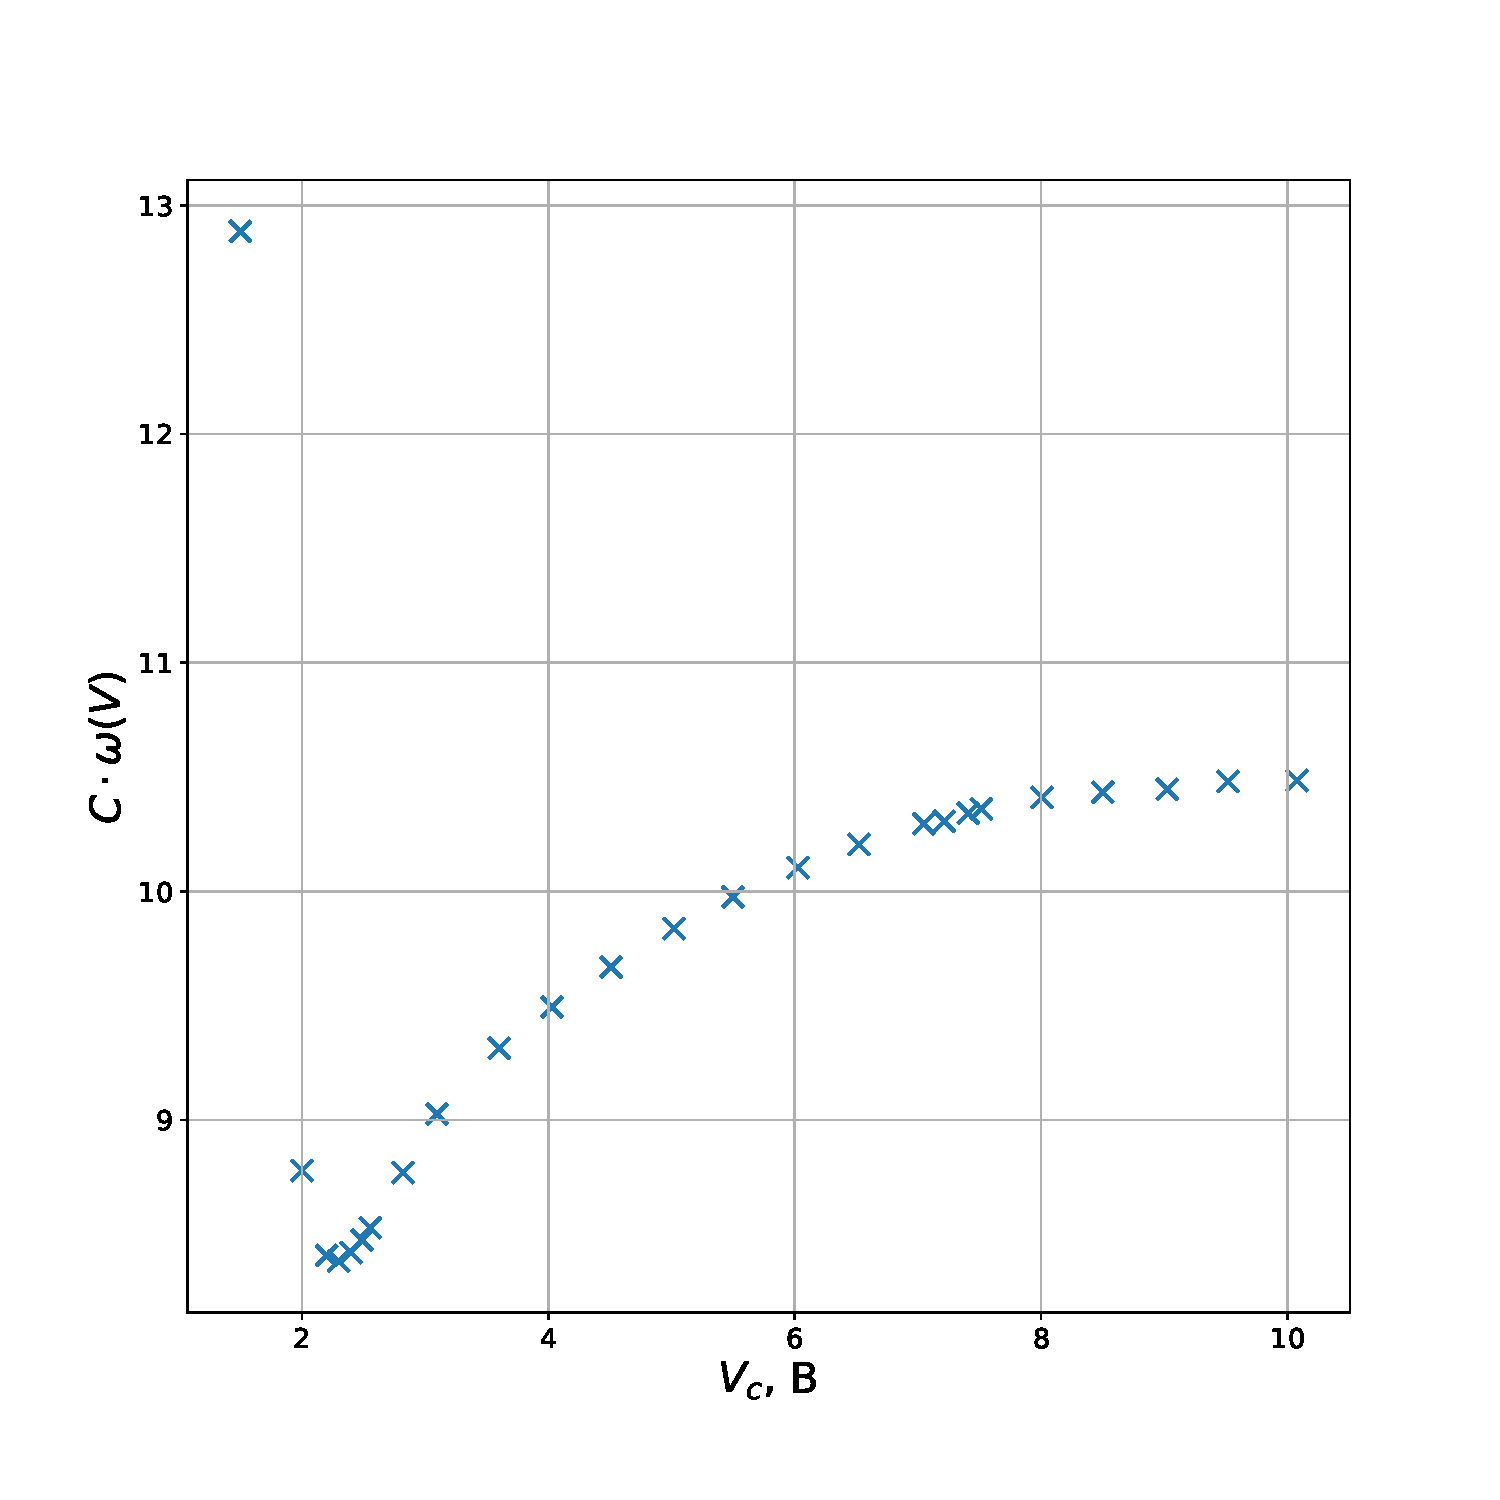
\includegraphics[scale = 0.36]{graph3}
    \centering
    \caption{$U_{нак} = 2.829$}
    \label{pic:graph3}
\end{figure}

\begin{figure}[!h]
    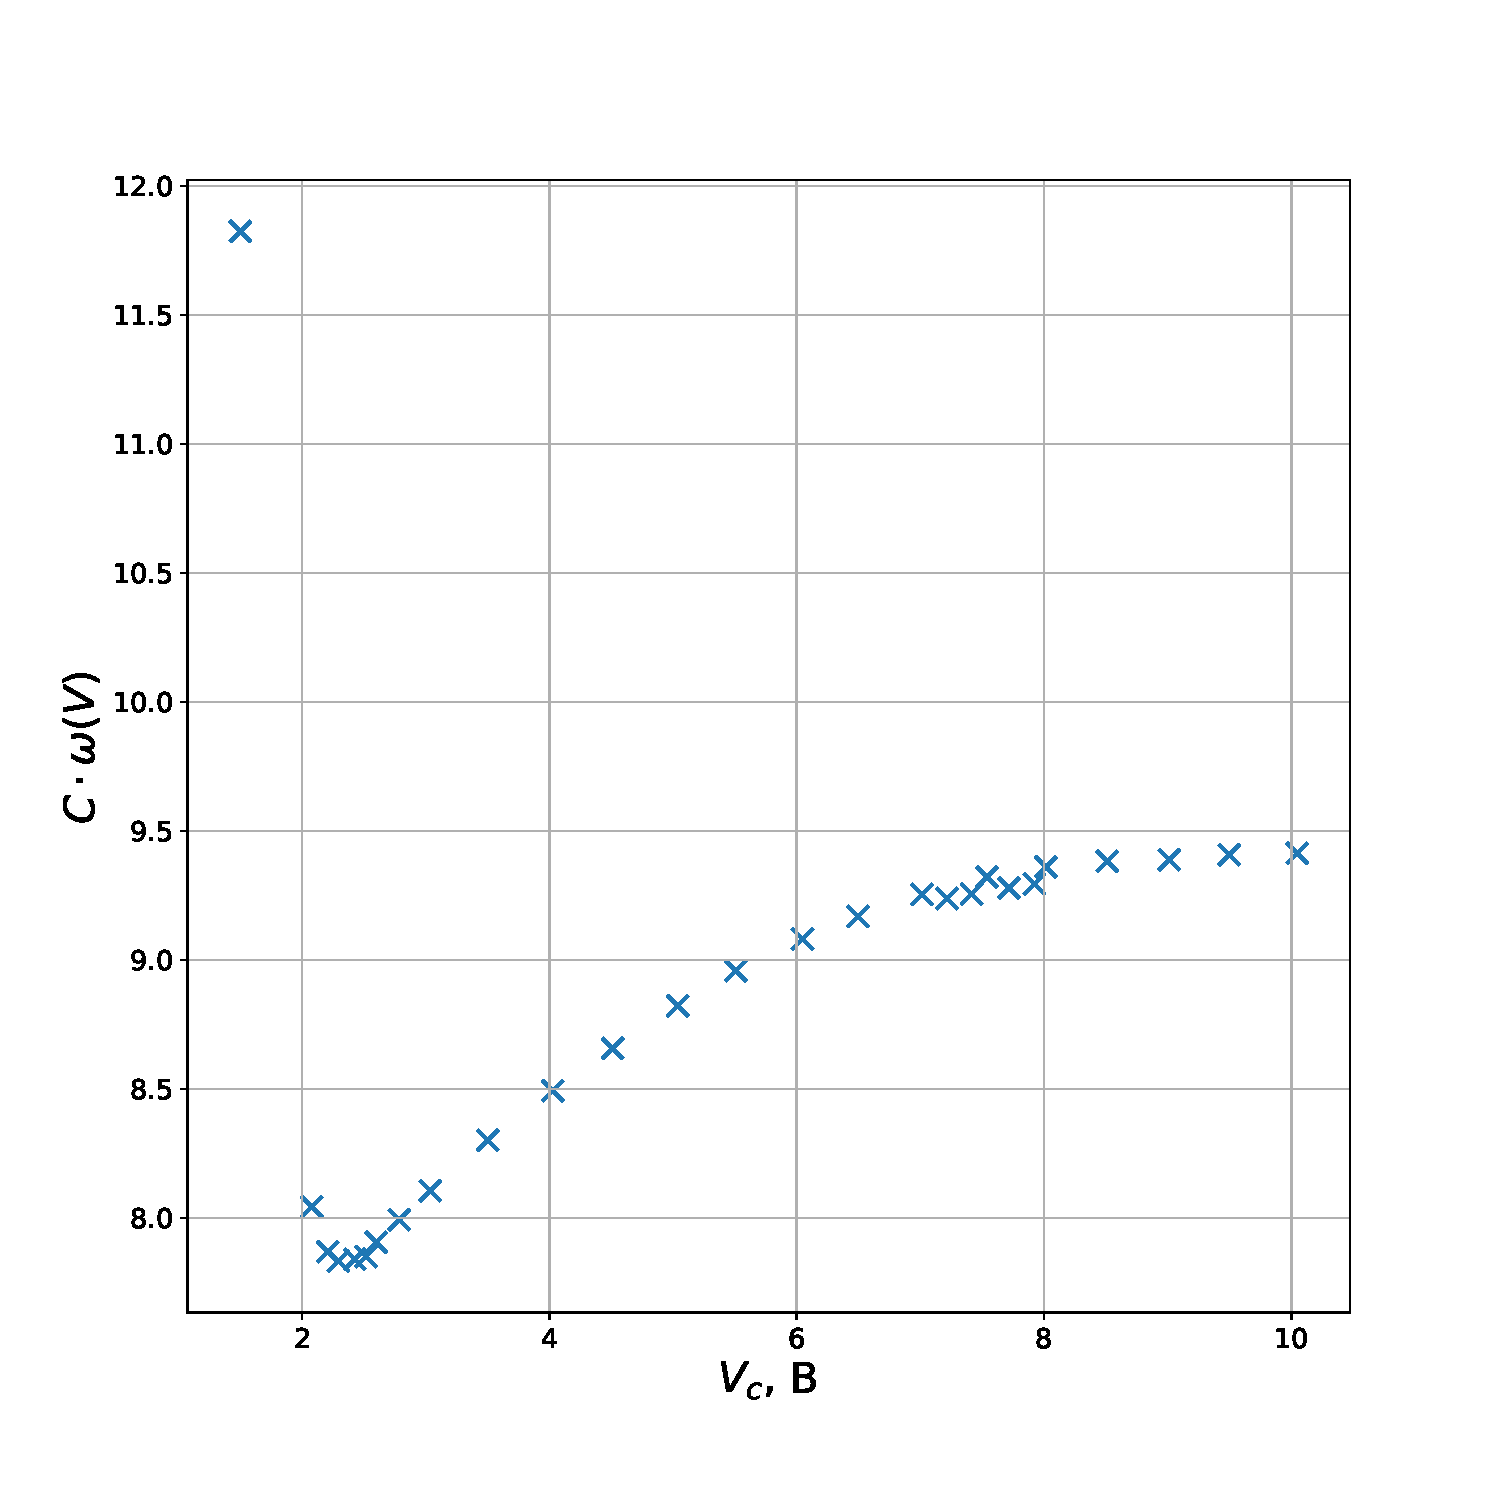
\includegraphics[scale = 0.4]{graph4}
    \centering
    \caption{$U_{нак} = 3.125$}
    \label{pic:graph4}
\end{figure}

\end {document}
